%THEORY
\chapter{Theory}
\label{chapter:theory}
% Innledning
XML is designed for encapsulation of structured and semistructured data,
relational data, and object repositories. The XQuery query language is designed
to perform flexible queries in such documents. A translation of such a
language to relational algebra requires detailed knowledge about XQuery for a
proper translation to be made. In this chapter, section
\ref{sect:theory:xquery} describes important details about the XQuery
language that are essential to this task. Further, existing implementations of
such translators are documented and compared.

Additionally, the concept of classic relational algebra itself is outlined in
section \ref{sect:theory:relAlg}, as the target algebra will be based on much
of its semantics.

Then in section \ref{sect:parser_and_syntaxtrees}, some common strategies for
parsing and construction of parser are outlined, as well as techniques for
parsing syntax trees.

Finally, a thoroughly researched method for translating XQuery to relational
algebra dubbed ``loop lifting'' is described in section
\ref{sect:theory:loop_lifting}.

\section{XQuery}
\label{sect:theory:xquery}

XQuery is a query language developed by the XML Query working group of W3C.
Version 1.0\cite{w3c00} became a W3C Recommendation January 2007. It was
designed as a response to an emerging task: to intelligently express queries in
the increasing amounts of information stored, exchanged and presented using
XML. The language is derived from Quilt\cite{quilt_queryLanguage}. Development
of XQuery 1.0 was coordinated with the development of XSLT 2.0, and the two
teams cooperated on development of XPath 2.0.

XQuery can be used to query any kind of data structure that can be represented
as an XML document. This includes text documents, relational databases and XML-compliant HTML markup.

\subsection{Basic language features}
\label{sect:theory:xquery:basics}
XQuery is a functional language with a comparatively small syntax. It lacks
some features known from many functional languages, such as support for higher
order function declarations.\marginpar{vet ikke hva higher order function declarations er jeg, hva skjer med
external?} However, it has some of the most important benefits, such as a lack of side-effects. XQuery is a
\textit{declarative} language (as opposed to \textit{imperative} languages), and
is strongly typed. Static typing is optional, and may vary between various
implementations.


XQuery is an orthogonal language, meaning that most expressions can be
arbitrarily nested. For example, a path expression predicate can be another
path expression:
\begin{center}
\texttt{/a/b[/c/d[e]]}
\end{center}
Or, the return-clause in a loop construct can be another loop
construct:
\begin{center}
\begin{tabular}{l}
\texttt{for \$i in (1,2,3) } \\ \quad 
\texttt{return for \$j in (4,5,6)} \\ \quad\quad 
\texttt{return \$i + \$j}
\end{tabular}
\end{center}

These features are important to consider for later translation, as truth values
in predicates and return values may need to be coerced and/or inferred into
their proper types and values.

The XQuery type system is rather complex, and we refer to some of the
introductory articles\cite{rys_xq_type_intro} by Michael Rys, as well as the
XQuery formal semantics specification\cite{xquery_semantics} for more
information about this. However, we will emphasize some important traits about
the type system:

\textbf{All sequences are one-dimensional}. Any given sequence that is not
one-dimensional, will be flattened. For example, the two-dimensional sequence
\verb!((1,2),3)! is to be flatted into \verb!(1,2,3)!.

Sequences can evaluate to an effective boolean value. Informally, this value is defined as follows:
\textbf{Anything that is not 0, empty, or \textit{false}, evaluates to \textit{true}}. In a boolean context (such
as an predicate or an \texttt{if..then..else}), this means that anything that is ``something'' will evaluate to
\textit{true}.


\subsection{Path Expressions}
\label{sect:theory:xquery:PathExpressions}
XPath (XML Path Language) is a small language for traversing and selecting
nodes (both element nodes and text nodes) from XML data. XPath is a subset of
XQuery, and is also available in XSLT, XML Schemas, XForms, and several other
technologies related to XML. 

In its abbreviated form, XPath bears a strong resemblance to file path syntax
known from many modern operating systems. This implies that the XPath syntax
may be familiar and intuitive for new users.

For example, consider the following XML source:
\begin{center}
\begin{minipage}[h]{5.2cm}
\begin{verbatim}
<a>
  <b><c>Hello World</c></b>
</a>
\end{verbatim}
\end{minipage}
\end{center}
If we execute the XPath expression \verb!/a/b/c!, we will receive the
\verb!c!-node which is a child of the \verb!b!-node which is a child of the
\verb!a!-node which is the document root node. Note that we will \textit{not}
receive the text \texttt{Hello World}, which is a \textbf{text node}, but rather its
parent node, which is the \verb!c!-node. To retrieve the text, we would rather
use the path expression \verb!/a/b/c/text()!. The  \verb!text()! expression is
known as a \textbf{kind test}. The following kind tests are available:
\begin{itemize}
  \item \verb!text()! - as described above, returns a text node
  \item \verb!comment()! - returns a comment node, for example \texttt{<!-- Hello
  world -->}
  \item \verb!processing-instruction()! - returns processing instructions, which
  means constructs such as \texttt{<?xml version="1.0"?>}
  \item \verb!node()! - returns any type of node 
\end{itemize} 

In its unabbreviated syntax (or, verbose syntax), the semantics of XPath
become more clear. For the XML source above, the full syntax for the path
expression to match the \verb!c!-node would be
\texttt{/child::a/child::b/child::c}. Here we see a new addition to our path
expression, the \verb!child::! axis specifier. An \textbf{axis specifier} helps
navigation within the XML document, by allowing the user to specify further
traits about the nodes to be matched. For example, attribute nodes can be
matched using \verb!attribute::! (or \verb!@!, with abbreviated syntax). For a
complete reference to axis specifiers, we refer to \cite{w3c01}.

\subsection{Predicates}
\label{sect:theory:xquery:Predicates}
Predicates are used in path expressions to filter nodes. Predicates are
appended to step expressions (and filter expressions, see \cite{w3c01}), and multiple predicates
are applied from left to right. Predicates never add to the node sets returned from the path expressions, they
only restrict by filtering. Predicate expressions are appended to step expressions within square brackets, like
this:
\begin{center}
\verb!/a/b[@id > 1]!
\end{center} 
This expression will return all \verb!b!-nodes within a \verb!a!-node and with an attribute \verb!id! whose value
is larger than one.

Consider the following XML source:
\begin{center}
\begin{minipage}[h]{3.2cm}
\begin{verbatim}
<a>
  <b id="1">
    <c />
  </b>
  <b id="2">
    <c />
  </b>
</a>
\end{verbatim}
\end{minipage}
\end{center}
If we apply the path expression mentioned above, we will thus receive the second
\verb!b!-node.

There are a few important things to note about predicates. Firstly, the
predicate expression can be any expression, and as such its return value is
coerced into a effective boolean value (either \textit{true} or \textit{false}), as
described previously in section \ref{sect:theory:xquery:basics}.

However, there is one important exception -- if the return value for the
predicate expression evaluates to a numerical value, then the predicate
becomes a \textbf{numeric predicate}, and its value is used to identify the
\textit{n}th node in the step expression. For example, the following path
expression returns the first \verb!b!-node: \verb!/a/b[1]!. As it is the first \verb!b!-node within the only
\verb!a!-node. \texttt{/a/b/c[1]} will select both \verb!c!-nodes of the document as they both are the first
\texttt{c}-node within their respected \texttt{b}-nodes.

\subsection{FLWOR}
\label{sect:theory:xquery:Flwor}

\begin{myDefinition}
\label{definition:iteration_expression}
An \textbf{iteration expression} or \textbf{iterator} is an XQuery expression consisting of an \textbf{iterator
variable} declaration and an \textbf{iterator body}. The \textbf{iterator body} is executed multiple times, and
for each time the \textbf{iterator variable} is bound to the next item in the \textbf{iterator sequence}.
\end{myDefinition}

XQuery is centered around a loop construct known as FLWOR, which is an acronym:
\begin{itemize}
  \item \textbf{F}or - iteration over tuples
  \item \textbf{L}et - assignment of tuples
  \item \textbf{W}here - conditional expression
  \item \textbf{O}rder by - sorting 
  \item \textbf{R}eturn - return expressions (similar to yielding in coroutines
  known from functional languages, not to be confused with a return statement
  in languages such as Java)
\end{itemize}
The FLWOR construct is thought to be roughly equivalent to a
\texttt{SELECT}-statement in SQL. For example, consider the following SQL
statement: 
\begin{center}
\verb!SELECT v.title FROM video v WHERE v.year = 1999!
\end{center}
And then compare it to the following XQuery counterpart:
\begin{center}
\begin{tabular}{l}
\texttt{for \$v in doc("videos.xml")//video} \\
\texttt{where \$v/year = 1999}\\
\texttt{return \$v/title}\\
\end{tabular}
\end{center}
Then construct a file \texttt{videos.xml} with the following contents:
\begin{center}
\begin{minipage}[h]{9.5cm}
\begin{verbatim}
<videos>
  <video>
    <title>Plan 9 from outer space</title>
    <year>1959</year>
  </video>
  <video>
    <title>Earth vs. the Flying Saucers</title>
    <year>1956</year>
  </video>
</videos>
\end{verbatim}
\end{minipage}
\end{center}
And finally execute the above query on this file to receive the following
result:
\begin{center}
\begin{minipage}[h]{7.5cm}
\begin{verbatim}
<title>Plan 9 from outer space</title>
\end{verbatim}
\end{minipage}
\end{center}
It is important to note the distinction of bound and free variables in FLWOR
constructs -- or, in other words, the scope boundaries. Consider the following
example:
\begin{center}
\begin{tabular}{l}
\texttt{for \$a in (1,2,3)} \\ \quad
  \texttt{return for \$b in (4,5,\$a)}\\ \quad\quad
    \texttt{return \$a + \$b}
\end{tabular}
\end{center}

When evaluating the for-clauses in this nested FLWOR expression, the
\textit{iterator sequence} is evaluated in the parent scope and not the
new scope for the current FLWOR expression. We can illustrate this point by
separating the scopes graphically:
\begin{figure*}
\centering
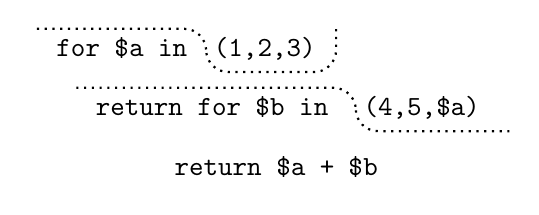
\begin{tikzpicture}
\node at (0,0) [label=right:\texttt{for \$a in}]{};
\node at (2,0) [label=right:\texttt{(1,2,3)}]{};
\node at (0.5,-0.75) [label=right:\texttt{return for \$b in}]{};
\node at (3.9,-0.75) [label=right:\texttt{(4,5,\$a)}]{};
\node at (1.5,-1.5) [label=right:\texttt{return \$a + \$b}]{};
\draw[thick,dotted,rounded corners=8pt]
(0,0.25) -- (2.15,0.25) -- (2.15,-0.3) -- (3.8,-0.3) -- (3.8,0.25) ;
\draw[thick,dotted,rounded corners=8pt]
(0.5,-0.5) -- (4.05,-0.5) -- (4.05,-1.05) -- (6,-1.05);
\end{tikzpicture}
\end{figure*}

As can be seen, the iterator sequence for the inner loop is evaluated in the
scope of the outer loop, and a new scope is not started until this iterator
sequence has been evaluated. Otherwise one could risk overwriting variables in
the iterator sequence when binding variables in the new scope.

Furthermore, a FLWOR construct may consist of several \texttt{for}- and
\texttt{let}-clauses in any order -- and each of these clauses may contain
several variable bindings. For example, the following is a valid XQuery
FLWOR expression:

\begin{center}
\begin{tabular}{l}
\texttt{for \$a in (1,2), \$b in (3,4) let \$c := 5, \$d := 6} \\ \quad
  \texttt{return \$a + \$b + \$c + \$d} \\
\end{tabular}
\end{center}

However note that semantically this expression is equivalent to:

\begin{center}
\begin{tabular}{l}
\texttt{for \$a in (1,2) return} \\ \quad
  \texttt{for \$b in (3,4) return} \\ \quad \quad
    \texttt{let \$c := 5 return} \\ \quad \quad \quad 
      \texttt{let \$d := 6 return} \\ \quad \quad \quad \quad 
        \texttt{\$a + \$b + \$c + \$d} \\
\end{tabular}
\end{center}

The latter seems significantly less complex to parse, since this query embodies
no less than \emph{four} individual FLWOR expressions, each with one and only
one \texttt{for}- or \texttt{let}-clause. This raises the question, could it be
benefitial to rewrite complex FLWOR expressions into a simpler form? This
question is addressed in section \ref{sect:method:ast_rewrite} on page
\pageref{sect:method:ast_rewrite}.

\subsection{Full Text Extensions}
\label{sect:theory:xquery:fulltext_ext}
XQuery is by nature a structural query language -- that is, queries are based on
document/data structure and not on content. The full-text extensions to XQuery
reduces the smallest unit of an XML document to single words instead of nodes.
Additionally, they add sophisticated tools such as stemming, thesaurus, and
scoring variables.

Technically, the \verb!ftcontains! operator applies tokenisation of the first
operand, and searches for a match with the second operand among the tokens. It
allows specifying match options like stemming, thesaurus, etc to a second
operand modifying the criteria for finding a match. A full list of match
options are described in \cite{w3c01}.

For example, consider the following example:
\begin{center}
\begin{tabular}{l}
\texttt{for \$b in /books/book} \\
\texttt{where \$b/title ftcontains ("dog" with stemming case sensitive)} \\ \quad\quad\quad
\texttt{ftand "cat"} \\
\texttt{return \$b/author}
\end{tabular}
\end{center}
This will match any \texttt{book}-node where the \texttt{title}-node contains a word with the stem ``dog''.
Further, the word must be in lower case, and the word ``cat'' must reside inside the same node. The query will
return the \texttt{author}-node of these \texttt{book}-nodes. 

\subsection{XQuery Core}
\label{sect:theory:xquery:XQcore}
XQuery Core is a less powerful but semantically equivalent language for expressing
XQuery queries. XQuery Core as well as the process of normalising regular
XQuery to XQuery Core is described in the document ``XQuery 1.0 and XPath 2.0
Formal Semantics''\cite{xquery_semantics}.

The goal of this subset language is to simplify queries and remove syntactic sugar,
leaving only the essential semantics without loss of expressiveness.
This is useful for optimization routines and translations into new types of
queries, for example relational algebra or SQL.

The process of normalisation is described through a rich set of mapping
rules. These are documented in detail in \cite{xquery_semantics} and will not be reiterated here.
However we will examine some important examples.

First, however, it is important to take note of the syntax of the mapping
rules, as described in \cite{xquery_semantics}, section 3.2.2. 
 
\begin{figure}[!h]
  \centering
$
[Object]_{Subscript}, premises == Mapped Object
$
  \caption{Mapping rules syntax}
  \label{figure:xquery:mapping_rules}
\end{figure}

Consider figure \ref{figure:xquery:mapping_rules}. Here, the left-hand side of the
equality symbol (==) denotes the original object to be rewritten. The
subscript indicates the type or kind of the object to be mapped, and/or
additional information to be passed between mapping rules. The right-hand side
denotes the rewritten object.

\subsubsection{Rewriting FLWOR expressions}
\label{sect:theory:xquery:core:rewriting_flwor}
\begin{figure}[!h]
\centering
[\texttt{for \$}$VarName_1$ $OptTypeDeclaration_1$ $OptPositionalVar_1$ \texttt{in} $Expr_1$\texttt{,}
\ldots, \texttt{\$}$VarName_n$ $OptTypeDeclaration_n$ $OptPositionalVar_n$ \texttt{in} $Expr_n$
$FormalReturnClause]_{Expr}$ \newline
$==$ \newline
\texttt{for \$}$VarName_1$ $OptTypeDeclaration_1$
$OptPositionalVar_1$ \texttt{in} $[Expr_1]_{Expr}$ \texttt{return} \texttt{\ldots for \$}$VarName_n$
$OptTypeDeclaration_n$ $OptPositionalVar_n$ \texttt{in} $[Expr_n]_{Expr}$ \texttt{return}
$[FormalReturnClause]_{Expr}$
  \caption{XQuery FLWOR expression to XQuery Core mapping rule}
  \label{figure:xquery:flwor_mapping_rule}
\end{figure}

The mapping rule for FLWOR \texttt{for}-clause expressions can be seen in figure
\ref{figure:xquery:flwor_mapping_rule}. The mapping rule for \texttt{let}-expressions is
similar and omitted for brevity, however they are also normalised into several nested bindings.

\begin{figure}[!h]
\centering
$[$\texttt{where} $Expr_1 FormalReturnClause]_{Expr}$ \newline
$==$ \newline
\texttt{if(}$[Expr_1]_{Expr}$\texttt{) then }$[FormalReturnClause]_{Expr}$ \texttt{else ()}
  \caption{XQuery \texttt{Where}-clause to XQuery Core mapping rule}
  \label{figure:xquery:where_mapping_rule}
\end{figure}

\begin{figure}[!h]
\centering
$[$\texttt{stable}$?$ \texttt{order by} $OrderSpecList FormalReturnClause]_{Expr}$ \newline
$==$ \newline
$[OrderSpecList]_{OrderSpecList}$\texttt{ return }$[FormalReturnClause]_{Expr}$
  \caption{XQuery \texttt{order by}-clause to XQuery Core mapping rule}
  \label{figure:xquery:orderby_mapping_rule}
\end{figure}

\begin{figure}[!h]
\centering
$[$\texttt{return }$Expr]_{Expr}$ \newline
$==$ \newline
$[Expr]_{Expr}$
  \caption{XQuery \texttt{return} clause to XQuery Core mapping rule}
  \label{figure:xquery:return_mapping_rule}
\end{figure}

Similarly, the mapping rules for \texttt{where}-clauses, \texttt{order by}-clauses and
\texttt{return}-clauses can be seen in figures \ref{figure:xquery:where_mapping_rule},
\ref{figure:xquery:orderby_mapping_rule},
and \ref{figure:xquery:return_mapping_rule}.

For an example of how these rules are applied, consider the following FLWOR
expression:
%\verbatiminput{graph_queries/flwor_rewrite1.xq}
\begin{center}
\begin{tabular}{l}
\texttt{for \$i in (1, 2), \$j in (3, 4)} \\
  \texttt{let \$k := \$i + \$j} \\
  \texttt{where \$k >= 5} \\
   \texttt{return (\$i, \$j)} \\
\end{tabular}
\end{center}

By applying the mapping rules described,  this expression is typically
rewritten to:
%\verbatiminput{graph_queries/flwor_rewrite2.xq}
\begin{center}
\begin{tabular}{l}
\texttt{for \$i in (1, 2) return} \\ \quad
  \texttt{for \$j in (3, 4) return} \\ \quad
    \texttt{let \$k := \$i + \$j return} \\ \quad \quad
      \texttt{if (\$k >= 5) then} \\ \quad \quad \quad
        \texttt{(\$i, \$j)}\\ \quad \quad
      \texttt{else} \\ \quad \quad \quad
        \texttt{()}
\end{tabular}
\end{center}
The corresponding AST graphs can be seen in figures
\ref{tree:ast:flwor_rewrite1} and \ref{tree:ast:flwor_rewrite2}. In particular,
note that multiple \texttt{for}-clauses in a FLWOR expression is rewritten into several
nested FLWOR expressions, and that the \texttt{where}-clause is  rewritten into an
\texttt{if..then..else} expression. 
\newpage
\begin{figure}
\centering
\subfigure[FLWOR AST tree before normalisation]{
 \includegraphics[scale=0.4]{img/graphs/flwor_rewrite1}
\label{tree:ast:flwor_rewrite1}
}
\subfigure[Normalised FLWOR AST tree]{
 \includegraphics[scale=0.4]{img/graphs/flwor_rewrite2}
\label{tree:ast:flwor_rewrite2}
}
\caption{A FLWOR expression before and after normalisation.}
\end{figure}

\subsubsection{Rewriting composite relative path expressions}
A composite relative path expression (for example, \verb!a/b!), can be
rewritten into a \texttt{for}-loop using the mapping rule in
\ref{figure:xquery:relpath_mapping_rule}.

\begin{figure}[!h]
\centering
$[RelativePathExpr / StepExpr]_{Expr}$ \newline
$==$ \newline
\begin{tabular}{l}
\texttt{fs:apply-ordering-mode(} \\ \quad
\texttt{fs:distinct-doc-order-or-atomic-sequence(} \\ \quad\quad
    \texttt{let} \texttt{\$fs:sequence as node()* :=} $[RelativePathExpr]_{Expr}$ \texttt{return} \\\quad\quad
    \texttt{let \$fs:last := fn:count(\$fs:sequence) return} \\\quad\quad
    \texttt{for \$fs:dot at \$fs:position in \$fs:sequence return} \\\quad\quad\quad\quad\quad
       $[StepExpr]_{Expr}$ \texttt{))}
       \end{tabular}
  \caption{Composite relative path expression mapping rule}
  \label{figure:xquery:relpath_mapping_rule}
\end{figure}

Given the trivial example \verb!a/b!, this translates into the following block
of normalised code:
\begin{center}
\begin{minipage}[h]{10cm}
\begin{verbatim}
fs:apply-ordering-mode (
fs:distinct-doc-order-or-atomic-sequence (
  let $fs:sequence as node()* := a return
  let $fs:last := fn:count($fs:sequence) return
  for $fs:dot at $fs:position in $fs:sequence return
    b))
\end{verbatim}
\end{minipage}
\end{center}


Which may seem like a rather verbose representation of such a simple path
expression. In particular, for complex path expressions this may
escalate into rather large rewritten expressions. However, this is a trade-off
to be made for normalisation of such path expressions.


% \subsection{AllMatches}
% \label{sect:theory:xquery:allmatches}
% \begin{itemize}
%   \item http://www.w3.org/TR/xpath-full-text-10/\#AllMatchesSec
%   \item Hva er AllMatches?
%   \item Kobling til fulltekst
%   \item Noen eksempler
%   \item Den store forskjellen med AllMatches er at den minste enheten i et 
%         dokument er et ord og ikke en tekstnode
% \end{itemize}
% om hvis vi bare ignorerer fulltekst uansett. Kunne foreslaatt en tilnarming ala galatex kanskje, som bare
% oversetter greiene til funksjonskall.

% State of the art, nåværende teknologi og implementasjoner
\section{Current state of XQuery}
\subsection{General}
\subsection{Implementations with full-text extensions}
\subsubsection{Quark / TexQuery}
%Relasjonsalgebra
\section{Relational Algebra}
\label{sect:theory:relAlg}

The relational model for database management was introduced for the first time by Edgar Frank Coddin 1974
(\cite{TDT4225}). It was based on relational algebra which is an offshoot of first-order logic. Several terms are
used when talking about relational algebra (\cite{gordonRussel, newYorkDB, sudarshan}):
\begin{itemize}
\item Set: A mathematical definition for a collection of objects which contains no duplicates
\item Domain: A \textit{set} of atomic values
\item Attribute: A real world role played by a named \textit{domain}
\item Tuple: A collection of \textit{attributes} which describe some real world entity
\item Relation: A \textit{set} of \textit{tuples}
\item Degree: The number of \textit{attributes} a \textit{relation} contains. Sometimes called arity.
\item Cardinality: The number of \textit{tuples} in a \textit{relation}
\item Union compatible: Two relations R and S are union compatible if and only if they have the same
	\textit{degree} and the \textit{domains} of the corresponding \textit{attributes} are the same.
\end{itemize}

\subsection{Primary Operators}
\label{sect:theory:relAlg:primOper}
The primary operators is a set of operators which constitutes the base of an algebra. Other operators can be
defined in terms of the primary ones. If one of the primary operators is excluded, the algebra will loose some of
it's expressiveness. The primitive operators of Codd's algebra are: selection, projection, union, difference,
cross product and rename (later added for the sake of the named relational algebra).

\subsubsection{Selection}
\label{sect:theory:relAlg:selection}
Selection is a unary operator, and is used to obtain a subset of the tuples of a relation that satisfy a select
condition. The resulting relation may have fewer tuples but it will have the same degree as the original relation.
It is sometimes called restriction to avoid confusion with SELECT in SQL. The operator is often symbolized by
\emph{s}igma:
\begin{equation*}
\sigma_{C}(R)
\end{equation*}
Where $R$ is a relation and $C$ is the select condition: a truth value or an expression yielding a truth value.
The expression can be made up of any combination of the logical operators \begin{math}\{ \wedge, \vee,
\neg\}\end{math}. Figure \ref{fig:theory:select} shows an example of a select operation.

\begin{figure}[h]
\centering
\begin{tabular}{lcr}
		\begin{tabular}{|c|c|} \hline
			\multicolumn{2}{|c|}{\textbf{R}} \\ \hline
			\textbf{Letter} & \textbf{Number} \\ \hline
			A & 1 \\ \hline
			A & 3 \\ \hline
			A & 6 \\ \hline
			B & 7 \\ \hline
		\end{tabular}  &
		\begin{math} \sigma _{Letter='A' \wedge Number > 2}(R) = \end{math}
		\begin{tabular}{|c|c|} \hline
			\multicolumn{2}{|c|}{} \\ \hline
			\textbf{Letter} & \textbf{Number} \\ \hline
			A & 3 \\ \hline
			A & 6 \\ \hline
		\end{tabular} 

\end{tabular}
\caption{Example showing the selection operator}
\label{fig:theory:select}
\end{figure}

\subsubsection{Projection}
\label{sect:theory:relAlg:projection}
Projection is also a unary operator, and is used to obtain a subset of the attributes of a relation. The resulting
relation will have an equal or lower degree than the original relation. In the case of duplicates being produced
as a result of omitting some attributes, the resulting relation will have fewer tuples than the original.
\emph{P}i is often used to symbolize the operation:
\begin{equation*}
\pi _{attr}(R)
\end{equation*}
Where $R$ is a relation and $attr$ is the set of attributes to be returned from $R$. Figure
\ref{fig:theory:project} shows an example of a projection. \begin{figure}[h]
\centering
\begin{tabular}{lcr}
	\begin{tabular}{|c|c|c|} \hline
	\multicolumn{3}{|c|}{\textbf{R}} \\ \hline
	\textbf{Let} & \textbf{Num} & \textbf{Sym} \\ \hline
	A & 1 & \% \\ \hline
	B & 1 & \% \\ \hline
	C & 3 & \# \\ \hline
	\end{tabular} &
	\begin{math} \pi _{Num, Sym} (R) = \end{math}
	\begin{tabular}{|c|c|} \hline
	\multicolumn{2}{|c|}{} \\ \hline
	\textbf{Num} & \textbf{Sym} \\ \hline
	1 & \% \\ \hline
	3 & \# \\ \hline
	\end{tabular}
\end{tabular}	
\caption{Exaple showing the projection operator}
\label{fig:theory:project}
\end{figure}

\subsubsection{Union and Difference}
\label{sect:theory:relAlg:unionAndDiff}
Union and difference are two binary operators analogous with union and difference operators in set theory. The
relational algebra version of the operators requires that the relations involved are union compatible.

The union of two relations returns a relation which includes all the tuples that are in either or both of the
original relations. As the result is also a relation, any potential duplicates will be removed. The operation is
commutative, and the returned relation will have the same degree as the two relations involved. A union between
two relations are often symbolized thus:
\begin{equation*}
R \cup S
\end{equation*}
Where $R$ and $S$ are relations.

The difference of two relations R and S is a relation that contains all the tuples that are in R but not in S. The
returned relation will, as was the case with union, have the same degree as the two relations involved. A
difference between relations $R$ and $S$ is written like this:
\begin{equation*}
R - S 
\end{equation*}

\subsubsection{Cross Product}
\label{sect:theory:relAlg:crossProduct}
The cross product operator is sometimes referred to as the cartesian product operator. As with union and
difference, it also stems from set theory. The operator is used to combine all tuples in one relation with all the
tuples from another. The returned relation will have a degree equal the sum of the degrees of each of the original
relations, and a cardinality equal the product of the cardinalities. The operator is commutative and written as a
cross:
\begin{equation*}
R \times S = S \times R
\end{equation*}
Where $R$ and $S$ are relations. Figure \ref{fig:theory:crossproduct} shows an
example of a cross product. \begin{figure}[h]
\begin{tabular}{ccccc}
	\begin{tabular}{|c|} \hline
	\textbf{R} \\ \hline
	\textbf{Let} \\ \hline
	A \\ \hline
	B \\ \hline
	\end{tabular}
	&
	\begin{math} \times \end{math}
	&
	\begin{tabular}{|c|c|} \hline
	\multicolumn{2}{|c|}{\textbf{S}} \\ \hline
	\textbf{Num} & \textbf{Let} \\ \hline
	1 & C \\ \hline
	2 & A \\ \hline
	\end{tabular}
	&
	\begin{math} = \end{math}
	&
	\begin{tabular}{|c|c|c|} \hline
	\multicolumn{3}{|c|}{} \\ \hline
	\textbf{R.Let} & \textbf{S.Num} & \textbf{S.Let} \\ \hline
	A & 1 & C \\ \hline
	A & 2 & C \\ \hline
	B & 1 & C \\ \hline
	B & 2 & A \\ \hline
	\end{tabular}
\end{tabular}
\centering
\caption{An example of cross product.}
\label{fig:theory:crossproduct}
\end{figure}

\subsubsection{Rename}
\label{sect:theory:relAlg:rename}
Rename is a unary operator used to rename a relation and/or a subset of its attributes. The resulting relation
will be equal to the original one in all aspects except maybe some of its name properties. The Greek letter
\emph{r}ho is often used to mark the presence of the rename operator:
\begin{equation*}
\rho _{S}(R)
\end{equation*}
Where $R$ is the relation being renamed, and $S$ is a relational scheme. $S$ is on the form $T _{(a _{1},...a
_{n})}$ for a n-degree relation, where $T$ is the new relation name and $a _{1},...a _{n}$ is the new names for
relation $R$'s attributes from $1$ to $n$. The degree of the scheme must be the same as the degree of the relation
being operated on.

\subsection{Derived Operators}
\label{sect:theory:relAlg:derivedOper}
None of the six primary operators can be expressed as a combination of any of the others. In contrast, some useful
operators can be derived using one or more of the primary ones. Most notably among these are intersection and join.

\subsubsection{Intersection}
\label{sect:theory:relAlg:intersection}
Intersection is the fourth mentioned operator that stems from set theory. It is a binary operator, and the
resulting relation will contain the set of tuples that are in both of the relations operated on. It can be
expressed with the help of the difference operator, and hence require that the input relations are union compatible:
\begin{equation*}
R \cup S = R-(R-S)
\end{equation*}

\subsubsection{Joins}
\label{sect:theory:relAlg:joins}
Joins are a group of operators that all are derived from the primary operators with the cross product as a base.
Among the operators in this group is natural join, theta-join, equi-join, anti-join, semi-join, outer joins and
division. Some of these will be presented in this section.

\paragraph{Natural Join.}
\label{sect:theory:relAlg:naturalJoin}
Natural join is a binary operator that returns a relation consisting of all combinations of tuples in input
relations that are equal on their common attribute names. The result relation will have a degree equal to the sum
of the degrees of the two original relations subtracted the number of common attributes. It is possible to express
natural join as a combination of cross product, projection and selection:

\begin{equation*}
R \bowtie S = \pi_{a_{1},..., a_{n},R.b_{1},...,R.b_{n},c_{1},...,c_{n}}( \sigma _{R.b_{1}=S.b_{1} \wedge ... \wedge R.b_{n}=S.b_{n}}(R \times S))
\end{equation*}

Where $R$ and $S$ are relations, $b_{1},..,b_{n}$ are the common attributes, $a_{1},..,a_{m}$ are the attributes
unique to $R$ and $c_{1},...,c_{k}$ are the attributes unique to $S$. A rename operator can lastly be used to
remove the prefix of the common attributes.

\paragraph{Equi-join and Theta-join.}
\label{sect:theory:relAlg:equiAndThetaJoin}
Theta-join returns a relation which is a combination of all the tuples in the two input relations that satisfy a
condition $C$. $C$ is in the form $a \theta b$, where $a$ is a attribute name from one relation, $b$ is an
attribute from the other and $ \theta $ is a binary operator in the set $ \{ <, \leq , =, \geq , >  \} $. An
equi-join is a theta-join where the binary operator in the condition is the equality operator. Theta-join can be
expressed as a combination of select and cross product:

\begin{equation*}
R \bowtie _{a \theta b}S = \sigma _{a \theta b}(R \times S)
\end{equation*}

\paragraph{Division.}
\label{sect:theory:relAlg:division}
Division in relational algebra can be described as the inverse operator of cross product, in the same way division
and multiplication are inverse in natural numbers calculus -- i.e. they are not inverse if the division gives a
residue:

\begin{equation*}
(R \times S) \div R = S ~~and~~ (R \times S) \div S = R
\end{equation*}

The resulting relation after a division contains the attribute values of the divisor relation that are associated
with every member of the dividend relation (\cite{makeDiv}). The operation may be better explained as a
combination of cross product, projection and difference:

\begin{equation*}
R \div S = \pi _{a_{1},...,a_{n}}(R) - \pi _{a_{1},...,a_{n}}((\pi _{a_{1},...,a_{n}}(R) \times S) - R)
\end{equation*}

Where $R$ and $S$ are relations and $a_{1},...,a_{n}$ are the attributes unique to $R$.

\paragraph{Semi-join.}
\label{sect:theory:relAlg:semiJoin}
Semi-join is a binary operation which returns a relation with the attributes of the first relation, and all the
tuples in this same relation for which there is a tuple in the second relation that is equal on their common
attributes. Semi-join can be described with the projection and natural-join operators:

\begin{equation*}
R \ltimes S = \pi _{a_{1},...,a_{n}}(R \bowtie S)
\end{equation*}

Where $R$ and $S$ are relations, and $a_{1},...,a_{n}$ are the attributes unique to $R$.

\paragraph{Anti-join.}
\label{sect:theory:relAlg:antiJoin}
The anti-join operator is very similar to the semi-join operator (and is also sometimes referred to as the
anti-semi-join), except that it returns all the tuples in the first relation for which there is not a tuple in the
other relation on their common attributes. It can be described with help of semi-join and difference:

\begin{equation*}
R \rhd S = R - R \ltimes S
\end{equation*}

Where $R$ and $S$ are relations.

\paragraph{Outer Joins.}
\label{sect:theory:relAlg:outerJoin}
The outer joins works in many ways as the natural join, except the resulting relation will include some extra
tuples based on one or both of the input relations. The right outer join $(\times=)$ will return a relation with
all the tuples from a natural join between the first (left) and the second (right) relation, but also the tuples
from the right relation that did not match any tuples from the left one on their common attributes. These extra
tuples will have the value NULL in the result relation for all attributes that were unique to the left one. The
left outer join $(=\times)$ is analogous with the right version, the only difference is that the extra tuples will
be based on the left input relation. The result relation of a full outer join $(=\times=)$ will have extra tuples
based the ones that did not find a match in both input relations.

\section{Parsers and syntax trees}
\label{sect:parser_and_syntaxtrees}
Intro: basic parser prerequisites

\begin{itemize}
  \item Kort om forskjellige parser-teknologier
  \item Hvordan parseren vaar fungerer
  \item Hvordan ASTen ser ut\ldots kanskje nesten en egen subsection til
  dette.. iallefall i generelle trekk? hmmmmmz
  \item Syntax-tr\ae r og tre-parsing
\end{itemize}

\section{Loop Lifting}
\label{sect:translation:loop_lifting}
Loop lifting is a method of translating XQuery iteration expressions into relational algebra. The method was
developed by Torsten Grust and Jens Teubner and originally presented in \cite{pathfinder_mothertongue}. It is a
part of the Pathfinder project\cite{pathfinderHome} (see section \ref{sect:theory:pathfinder}).

In this section we will present Loop Lifting mainly based on the two articles \cite{pathfinder_mothertongue} and
\cite{pathfinder_purelyRelational}. The articles present the method for a subset of XQuery Core (Pathfinder
rewrites queries to Core, see section \ref{sect:theory:pathfinder}), of which we will only present the elements
relevant in a comparison between Loop Lifting and \underline{\textbf{\Large TODO:}} ``insertName''. Thus, the
translation of path expressions and XML-element construction will not be handled, as pathfinder's XML-tree
representation(section \ref{sect:theory:pathfinder}) is incompatible with Mars.

\underline{\textbf{\Large TODO:}}
\begin{itemize}
  \item peep hole plan simplification
  \item forutsetter det \aa~ jobbe p\aa~ DAGz? B\o r iallefalll gj\o re det, mye som blir brukt om igjen\ldots
\end{itemize}

\subsection{Operators}
\label{sect:translation:ll:Operators}
Loop-lifting utilises a set of relational algebra operators, out of which the ones used in this chapter is
presented in table \ref{tab:translation:llOperators}.
\begin{table}[h]
\centering
\begin{tabular}{l|l} 
$\pi_{a_{1}:b_{1},\ldots,a_{n}:b_{n}}$ 	& projection and renaming	\\ 	\hline
$\sigma_{a}$					   		& selection             	\\ 	\hline
$\dot\cup$ 							& disjoint union			\\	\hline
$\times$								& cartesian product			\\	\hline
$\bowtie_{a=b}$							& equi-join					\\ 	\hline
$\varrho_{b:(a_{1},\ldots,a_{n})/p}$	& numbering operator		\\	\hline
$\circledcirc_{b:(a_{1},\ldots,a_{n})}$	& $n$-ary arithmetic/comparison operator $\circ$ \\ \hline
\scriptsize \begin{tabular}{c|c} $a$& $b$\\\hline\end{tabular} & literal table
\end{tabular}
\caption[of the Pathfinder relational algebra]{Operators of the Pathfinder relational algebra. $a$, $b$ and $p$
represents attributes}
\label{tab:translation:llOperators}
\end{table}

Most of the operators are quite standard, and can easily be understood by comparing with the operators from
section \ref{sect:theory:relAlg} and \ref{sect:method:marsOperators}.

The selection operator ($\sigma_{a}$) selects tuples where attribute $a \ne 0$. Only a very restricted selection
is used, written $\sigma_{a}$, which only returns tuples satisfying $a \neq 0$.  Considering the numbering
operator, $p$ denotes the partitioning attribute, $(a_{1},\ldots,a_{n}$ the attributes to be sorted on and $b$ is
an added attribute holding the result of the
numbering. {\scriptsize{\begin{tabular}{c|c}$a$&$b$\\\hline\end{tabular}}}  represents the creation
of a relation with attributes $a$ and $b$.

Operator $\circledcirc_{b:(a_{1},\ldots,a_{n})}$ will evaluate the arithmetic/comparison expression $a_{1} \circ
\ldots \circ a_{n}$ and place the result in $b$. Where $\circ \in \left\{ +,- , <, =, \ldots  \right\} $.


\subsection{Basics}
\label{sect:translation:ll:Basics}
XQuery expressions evaluate to finite, ordered sequences of items. As a sequences are one-dimensional, it can be
represented by a single relation where each tuple encodes a sequence item. The order of the sequence is
maintained by an attribute \textit{pos}. The value of the item is held in an attribute \textit{item}. A sequence
such as \texttt{('a', 'b', 'c')} will be represented relationally like this:

\begin{center}
\begin{tabular}{|c|c|}\hline
\textit{pos}	& \textit{item} 	\\ \hline
1				& \texttt{'a'}		\\ \hline
2				& \texttt{'b'}		\\ \hline
3				& \texttt{'c'}		\\ \hline
\end{tabular}
\end{center}

For the rest of this chapter about Pathfinder's loop lifting, variables, expressions and scopes is denoted like
this (ref. section \ref{sect:theory:xquery:Flwor}):
\[
s \left\{
\begin{array}{l}
\qquad \qquad \quad \vdots \\
\mbox{\texttt{for \$}}v_{0}\mbox{\texttt{ in }} e_{0} \mbox{\texttt{ return}} \\
\quad s_{0} \left\{ e_{0}' \right. \\
\qquad \qquad \quad \vdots
\end{array}
\right.
\]

More generally, a scope $s_{x \cdot y}$ identifies the $y$th child scope of scope $x$, $x \in \left\{
\mathbb{N}\right\}, y \in \left\{ \mathbb{N} \right\}$. Expression $e_{x\cdot y}$ evaluates to an iterator sequence
and is bound to the variable $v_{x \cdot y}$. $e_{x \cdot y}'$ constitutes the coresponding iterator body, and $I_{x \cdot y}$ the whole iterator expression.

$q_{x}(e)$ is used to denote the relational representation of expression $e$ in scope $s_{x}$.


\subsection{Constant Subexpressions}
\label{sect:translation:ll:ConstExprs}

For a iterator expression $i_{x}$ with $n$ iterations there exists a relation $loop_{x}$, consisting of a
single column, \textit{iter}, with values 1,2,\ldots,$n$. In the outermost scope, $loop$ has a single tuple with
value 1.

A constant value $c$ in scope $s_{x}$ is \textit{lifted} is lifted like this:
\begin{equation}
q_{x}(c) =  loop_{x} \times \mbox{\scriptsize \begin{tabular}{c|c} \textit{pos}&\textit{item} \\
\hline 1 & \textit{c}
\end{tabular}}
\label{eq:ll:constLoopLift}
\end{equation}

A tuple ($iter,pos,item$) in a loop lifted relation for subexpression $e_{x}'$ can be understood as that during the
$iter$th iteration, the item in position $pos$ in $e_{x}'$ has the value $item$.

\subsection{Bound Variables}
\label{sect:translation:ll:boundVar}

A variable is bound
An iterator sequence expression $e_{x \cdot y}$ is evaulated in scope $s_{x}$. This sequence is then iterated over
and each item is successively bound to the iterator variable $v_{x \cdot y}$. The evaluation of $e_{x \cdot y}'$
is in scope $s_{x \cdot y}$ and utilises these bindings. 

Considering this, a representation of $v_{x \cdot y}$ in scope $s_{x \cdot y}$ may therefore be calculated by
retaining the values of $q_{x}(e_{x \cdot y})$, introducing a $iter$ attribute with consecutive numbers and
holding the $pos$ attribute to the constant value 1. In terms of algebra, the representation of $v_{x \cdot y}$ is
computed like this:
\begin{equation}
q_{x \cdot y}(\mbox{\texttt{\$}}v_{x \cdot y}) = \mbox{\scriptsize \begin{tabular}{c} $pos$ \\\hline 1
\end{tabular}} \times \pi_{iter:inner,item}(\varrho_{inner:(iter,pos)}(q_{x}(e_{x \cdot y})))
\label{eq:ll:qxy_vxy}
\end{equation}
The introduction of the $inner$ attribute is used to denote evaluation of the loop in scope $s_{x \cdot y}$. The
$iter$ attribute of $q_{x}(e_{x \cdot y})$ can be viewed as an atttribute $outer$, as it denotes the iterations in
the outer loop of scope $s_{x}$.

Loop lifting requires maintenance of a $loop$ relation ensuring independent iterations. The iterator body in
scope $s_{x \cdot y}$ needs to be evaluated once for each binding of the iterator variable $v_{x \cdot y}$.
Thus, the $loop$ relation needs to be redifined based on $q_{x \cdot y}(v_{x \cdot y})$:
\begin{equation}
loop_{x \cdot y} = \pi_{iter}(q_{x \cdot y}(v_{x \cdot y}))
\label{eq:ll:loopxy}
\end{equation}


\subsection{Free Variables}
\label{sect:translation:ll:freeVar}

XQuery expressions may use any iterator variable bound in enclosing scopes. That is, $v_{x}$ bound in
scope $s_{x}$ may also be referred to within any of its child scopes. When looking at one of these child scopes,
$s_{x \cdot y}$, by itself, the variable $v_{x \cdot y}$ appears to be a free variable.

Vision a iterator expresion $I_{x \cdot y}$ within another iterator expression $I_{x}$, both with iterator
sequences of length two. If $v_{x}$ is referred to within scope $s_{x \cdot y}$, from $s_{x \cdot y}$'s point of
view, $v_{x}$ is free. For each binding of $v_{x}$ in the \textit{outer} iteration expression, two
evaluations of the \textit{inner} iteration expresion occur. A relation capturing the relationship between number
of iterations of these two iterator expressions can be defined like this:
\begin{center}
\begin{tabular}{|c|c|}\hline
\textit{outer}	& \textit{inner} 	\\ \hline
1				& 1		\\ \hline
1				& 2		\\ \hline
2				& 3		\\ \hline
2				& 4		\\ \hline
\end{tabular}
\end{center}
Where a tuple $(outer, inner)$ is read as for the $inner$th iteration of the inner iterator expression, the outer
iterator expression is in its $outer$th iteration. This relation is called $map_{x, x\cdot y}$ as it maps
representations between scopes $s_{x}$ and $s_{x \cdot y}$. It can be calculated like this:
\begin{equation}
map_{x, x\cdot y} = \pi_{outer:iter,inner}(\varrho_{inner:(iter,pos)}(q_{x}(e_{x \cdot y})))
\label{eq:ll:mapx_xy}
\end{equation}

With this relationship defined it is now possible to represent the free variable $v_{x}$ in the scope $s_{x \cdot
y}$ with the help of an equi-join:
\begin{equation}
q_{x \cdot y}(\mbox{\texttt{\$}}v_{x}) = \pi_{iter:inner, pos,
item}(q_{x}\left(\mbox{\texttt{\$}}v_{x})\bowtie_{iter=outer} map_{x, x \cdot y}\right)
\label{eq:ll:qxy_vx}
\end{equation}

\subsection{Mapping Back}
\label{sect:translation:ll:mappingBack}

All steps and equations so far have been helpful to represent sequences and variables in a lower scope. But the
result of a query will have to be in form of its representation in the outermost scope $s$. So a way to represent
an expression $e_{x,y}'$ in its scope's parent scope $s_{x}$ is needed. Once again the $map$ relation may be of
use, combined with an equi-join:
\begin{equation}
q_{x}(e_{x \cdot y}') =
\begin{array}{l}
 \pi_{iter:outer, pos:pos1, item}(\\ \qquad\varrho_{pos1:(iter,pos)/outer}(q_{x \cdot
y}(e_{x \cdot y}')\bowtie_{iter = inner}map_{x, x \cdot y}))
\end{array}
\label{eq:ll:qx_exymark}
\end{equation}


\subsection{Other Expression Types}
\label{sect:translation:ll:OtherExpr}

The sequence construction \texttt{(}$e_{1}$\texttt{, }$e_{2}$\texttt{)} is essentially a disjont union of the
relational representations of the expressions, that is, $q_{x}(e_{1})$ and $q_{x}(e_{2})$. By temporarily adding a
attribute $ord$ to these relations before a renumbering of the result with $\varrho$, the proper ordering of the
sequence is aquired. Construction of sequences can therefore be expressed like this:
\begin{equation}
q_{x}(\mbox{\texttt{(}}e_{1}\mbox{\texttt{,}}e_{2}\mbox{\texttt{)}})=
\begin{array}{l}


\pi_{iter,pos:pos1,item}
\left( \right.\\ \qquad

\varrho_{pos1:(ord,pos)/iter}
	\left( \right. \\ \qquad \qquad
	\left. \left.
		\left(
		\frac{ord}{1} \times q_{x}(e_{1})
		\right)
		\dot\cup
		\left(
		\frac{ord}{1} \times q_{x}(e_{2})
		\right)		
	\right)
\right)
\end{array}
\label{eq:ll:secuence}
\end{equation}

The $\circledcirc$ operator meets the demand of evaluating comparison and arithmetic operations on atomic values.
Given two XQuery values $e_{1}$ and $e_{2}$ in multiple iterations, with relational representations as before,
the expression $e_{1}$ \texttt{ + } $e_{2}$ can be translated by first joining $q_{x}(e_{1})$ and $q_{x}(e_{2})$
on their iteration number, i.e. $iter$. Then, for each tuple, store the sum of the values of both of the $item$
attributes, before cleaning up the resulting relation with a project. Expressed as an equation, the sum expression looks like
this:
\begin{equation}
q_{x}(e_{1} \mbox{\texttt{ + }} e_{2}) =
\begin{array}{l}
\pi_{iter,pos,item:res}\left(\right. \\ \qquad
\oplus_{res:(item,item')}
\left( \right. \\ \qquad \qquad

	q_{x}(e_{1})
	\bowtie_{iter = iter'}
	 \\ \qquad \qquad \qquad
	\left.\left(\pi_{iter':iter, item':item}(q_{x}(e_{2}))
	\right)
\right)
\end{array}
\label{eq:ll:sumexpr}
\end{equation}

\subsection{Example}
\label{sect:translation:ll:example}

Only looking at equations may be a bit too abstact to fully understand the concept of loop lifting. To
concretise we will present a simple example of evaluating a query with the method and show intermediate results.
The naming of expressions, scopes and variables will, where possible, be the same as earlier in this chapter. This
query is the basis of this evaluation:

\begin{figure*}[h!]
\centering
\begin{math}
s\left\{
\begin{array}{l}
\mbox{\texttt{for \$v0 in (10,20) return}} \\ \;
s_{0}\left\{
\begin{array}{l}
\mbox{\texttt{(\$v0, for \$v00 in (7,8,9) return}} \\ \;
s_{0,0}\left\{ \mbox{\texttt{\$v0 + \$v00)}}\right.
\end{array}
\right.
\end{array}
\right.
\end{math}
\end{figure*}

The goal of the evaluation is, after all other calculations, to have a representation of $e_{0}'$ in scope $s$,
that is, $q(e_{0}')$. This is done by nesting inwards until the deepest scope, while calculating needed helping
relations on the way, before evaluating the subexpressions one by one as one nests outwards until the outermost
scope.

Firstly a representation of the outermost loop is needed. With the help of equation \ref{eq:ll:constLoopLift} we
find a representation of \texttt{(10, 20)} in scope $s$, $s(e_{0})$. Then, employing equation \ref{eq:ll:qxy_vxy}
yields \texttt{\$v0} in scope $s_{0}$, the result of which is shown in figure \ref{fig:translation:ll:q0_v0}.
$loop_{0}$ and $map_{\, ,0}$ can now be calculated by using equations \ref{eq:ll:loopxy} and \ref{eq:ll:mapx_xy}
and are shown in figure \ref{fig:translation:ll:loop0} and \ref{fig:translation:ll:map_0} respectevely (remember
$loop$ consists of a single tuple with value 1).

\begin{figure}[!h]
\centering
\subfigure[$q_{0}($\texttt{\$v0}$)$]{
%q0_v0
\begin{tabular}{|c|c|c|} \hline
$pos$	& $iter$	& $item$ \\ \hline
1		& 1			& 10 	\\ \hline
1		& 2			& 20 	\\ \hline
\end{tabular}
\label{fig:translation:ll:q0_v0}
%\caption{$q_{0}($ \texttt{\$v0} $)$}
}
\qquad \quad
\subfigure[$loop_{0}$]{

\begin{tabular}{|c|} \hline
$iter$ \\\hline
1 \\\hline
2 \\\hline
\end{tabular}
\label{fig:translation:ll:loop0}
%\caption{$loop_{0}$}
}
\qquad \quad
\subfigure[$map_{\, ,0}$]{
\begin{tabular}{|c|c|} \hline
$outer$ & $inner$ \\ \hline
1 & 1 \\ \hline
1 & 2 \\ \hline
\end{tabular}
\label{fig:translation:ll:map_0}
%\caption{$map_{\, ,0}$}
}
\label{fig:translation:ll:outerIntermediate}
\caption{Outer loop intermediate results}
\end{figure}

Before we evaluate the sequence expression in scope $s_0$, we need to evaluate the inner \texttt{for} loop. By the
same measure as with the outer loop we first calculate $q_{0\cdot 0}($\texttt{\$v00}$)$, $loop_{0 \cdot 0}$ and
$map_{0, 0 \cdot 0}$. The results are shown in figure \ref{fig:translation:ll:innerIntermediate}.

\begin{figure}[!h]
\centering
\subfigure[$q_{0\cdot 0}($\texttt{\$v00}$)$]{
\begin{tabular}{|c|c|c|} \hline
$pos$	& $iter$	& $item$ \\ \hline
1		& 1			& 7 	\\ \hline
1		& 2			& 8 	\\ \hline
1		& 3			& 9 	\\ \hline
1		& 4			& 7 	\\ \hline
1		& 5			& 8 	\\ \hline
1		& 6			& 9 	\\ \hline
\end{tabular}
\label{fig:translation:ll:q00_v00}
%\caption{$q_{0}($ \texttt{\$v0} $)$}
}
\qquad
\subfigure[$loop_{0 \cdot 0}$]{
\quad
\begin{tabular}{|c|} \hline
$iter$ \\\hline
1 \\\hline
2 \\\hline
3 \\\hline
4 \\\hline
5 \\\hline
6 \\\hline
\end{tabular}
\label{fig:translation:ll:loop00}
%\caption{$loop_{0}$}
\quad
}
\qquad 
\subfigure[$map_{0, 0 \cdot 0}$]{
\begin{tabular}{|c|c|} \hline
$outer$ & $inner$ \\ \hline
1 & 1 \\ \hline
1 & 2 \\ \hline
1 & 3 \\ \hline
2 & 4 \\ \hline
2 & 5 \\ \hline
2 & 6 \\ \hline
\end{tabular}
\label{fig:translation:ll:map0_00}
%\caption{$map_{\, ,0}$}
}
\caption{Inner loop intermediate results \label{fig:translation:ll:innerIntermediate}}
\end{figure}

To be able to calculate the sum-expression, $e_{0 \cdot 0}'$, we first need a representation of the variable
\texttt{\$v0} in scope $s_{0 \cdot 0}$. As this variable is a free variable in this scope, this is done by
applying equation \ref{eq:ll:qxy_vx} on $q_{0}($\texttt{\$v0}$)$ (figure \ref{fig:translation:ll:q0_v0}). This
result is shown in figure \ref{fig:translation:ll:q00_v0}. Now that we have both \texttt{\$v0} and \texttt{\$v00}
expressed from scope $s_{0 \cdot 0}$'s viewpoint, we can employ equation \ref{eq:ll:sumexpr} to sum the two variables together. The
resulting relation can be seen in figure \ref{fig:translation:ll:q00_e00m}.

\begin{figure}[!h]
\centering
\subfigure[$q_{0\cdot 0}($\texttt{\$v0}$)$]{
\qquad 
\begin{tabular}{|c|c|c|} \hline
$pos$	& $iter$	& $item$ \\ \hline
1		& 1			& 10 	\\ \hline
1		& 2			& 10	\\ \hline
1		& 3			& 10	\\ \hline
1		& 4			& 20	\\ \hline
1		& 5			& 20	\\ \hline
1		& 6			& 20	\\ \hline
\end{tabular}
\label{fig:translation:ll:q00_v0}
\qquad 
%\caption{$q_{0}($ \texttt{\$v0} $)$}
}
\subfigure[$q_{0\cdot 0}(e_{0\cdot0}')=q_{0\cdot 0}($\texttt{\$v0 + \$v00}$)$]{ 
\qquad 
\begin{tabular}{|c|c|c|} \hline
$pos$	& $iter$	& $item$ \\ \hline
1		& 1			& 17 	\\ \hline
1		& 2			& 18 	\\ \hline
1		& 3			& 19 	\\ \hline
1		& 4			& 27 	\\ \hline
1		& 5			& 28 	\\ \hline
1		& 6			& 29 	\\ \hline
\end{tabular}
\label{fig:translation:ll:q00_e00m}
\qquad
}
\caption{Innermost expression intermediate results \label{fig:translation:ll:innerExpr}}
\end{figure}

The result of the summation, $q_{0\cdot 0}(e_{0\cdot0}')$ is expressed in scope $s_{0 \cdot 0}$ and will have to
be mapped up to scope $s_{0}$. This is done with help from equation \ref{eq:ll:qx_exymark} and $map_{0, 0\cdot 0}$
which we calculated earlier, and the result can be seen in figure \ref{fig:translation:ll:q0_e00m}. With
$q_{0}(e_{0\cdot0}')$ evaluated, and with $q_{0}($\texttt{\$v0}$)$ from earlier, the sequence building can be completed. This operation requires
equation \ref{eq:ll:secuence}, and yields the relation shown in figure \ref{fig:translation:ll:q0_e0m}.

\begin{figure}[!h]
\centering
\subfigure[$q_{0}(e_{0\cdot0}')$]{
%q0_v0
\begin{tabular}{|c|c|c|} \hline
$pos$	& $iter$	& $item$ \\ \hline
1		& 1			& 17 	\\ \hline
2		& 1			& 18 	\\ \hline
3		& 1			& 19 	\\ \hline
1		& 2			& 27 	\\ \hline
2		& 2			& 28 	\\ \hline
3		& 2			& 29 	\\ \hline
\end{tabular}
\label{fig:translation:ll:q0_e00m}
%\caption{$q_{0}($ \texttt{\$v0} $)$}
}
\qquad
\subfigure[$q_{0}(e_{0}')$]{
\begin{tabular}{|c|c|c|} \hline
$pos$	& $iter$	& $item$ \\ \hline
1		& 1			& 10 	\\ \hline
2		& 1			& 17 	\\ \hline
3		& 1			& 18 	\\ \hline
4		& 1			& 19 	\\ \hline
1		& 2			& 20 	\\ \hline
2		& 2			& 27 	\\ \hline
3		& 2			& 28 	\\ \hline
4		& 2			& 29 	\\ \hline
\end{tabular}
\label{fig:translation:ll:q0_e0m}
%\caption{$loop_{0}$}
}
\qquad
\subfigure[$q(e_{0}')$]{
\begin{tabular}{|c|c|c|} \hline
$pos$	& $iter$	& $item$ \\ \hline
1		& 1			& 10 	\\ \hline
2		& 1			& 17 	\\ \hline
3		& 1			& 18 	\\ \hline
4		& 1			& 19 	\\ \hline
5		& 1			& 20 	\\ \hline
6		& 1			& 27 	\\ \hline
7		& 1			& 28 	\\ \hline
8		& 1			& 29 	\\ \hline\end{tabular}
\label{fig:translation:ll:q_e0m}
%\caption{$map_{\, ,0}$}
}
\label{fig:translation:ll:endExample}
\caption{Intermediate and final result}
\end{figure}

Finally the built sequence will have to be expressed in terms of scope $s$. Achieving this only requires the use
of equation \ref{eq:ll:qx_exymark} one last time in combination with $map_{ ,0}$. The complete result of the query
is shown in figure \ref{fig:translation:ll:q_e0m}.

\underline{\textbf{\LARGE TODO:}} ser at det trengs DAGz ja\ldots (?)

\section{Summary}
\label{sect:theory:summary}
\begin{itemize}
  \item sammendrag av dette kap
\end{itemize}